%%%%%%%%%%%%%%%%%%%%%%%%%%%%%%%%%%%%%%%%%%%%%%%%%%%%%%%%%%%%%%%
%         Estudio empírico de las funciones de activación
%%%%%%
%   1. Comparativas en cuanto a coste computacional.
%%%%%%%%%%%%%%%%%%%%%%%%%%%%%%%%%%%%%%%%%%%%%%%%%%%%%%%%%%%%%%%

\chapter{Funciones de activación}
\label{funciones-activacion-democraticas-mas-demoscraticas}
Como se observó en 
\ref{def:funcion_activacion_articulo}
se desconoce teóricamente si una función de activación va a ser 
mejor que otra, es por ello y puesto que nuestro objetivo 
es reducir el coste computacional de una red neuronal
que procederemos a realizar un análisis del costo de las redes neuronales. 


\section{Caracterización de las funciones de activación}  

Si bien por conveniencia teórica definimos las funciones de activación en \ref{def:funcion_activacion_articulo}
como una función de $\phi:\R \longrightarrow [0,1]$, no 
decreciente, con uno como límite en infinito y cero como límite a 
menos infinito. 

Nos basaremos en el concepto actual de función de activación,
basta con que sea una función no polinómica
(véanse  los artículos \cite{DBLP:journals/corr/SonodaM15}, \cite{modern-trainable-activation-functions} y \cite{FUNAHASHI1989183}),
además también incluiremos la función de activación identidad.

Funciones no polinómicas hay infinitas y reincidimos en que a priori no hay una mejor que otra; por tanto, como criterio de selección nos guiaremos por la intuición que nos brinda la demostración del teorema \ref{teorema:2_3_uniformemente_denso_compactos}.
  La imagen de una función de activación es relevante a la hora de aproximar la función ideal desconocida, ya que reduce el número 
  de neuronas si se usa convenientemente.  
Por lo tanto, una buena heurística sería disponer de un repertorio básico de funciones de activación que contemplen distintas imágenes no polinómicas. 

Además de las propuestas en \ref{def:funcion_activacion_articulo}, 
añadimos a nuestra colección las siguientes. 


\begin{table}[H] 
    \centering  
    \resizebox{\textwidth}{!}{
    \begin{tabular}{| c | c | c | c |}
        \hline
        Nombre & Expresión & Rango imagen  & Gráfica \\
        \hline
        %%%%%%%% Identidad %%%%%%%
        % Nombre: 
        Identidad 
        & %expresión 
        $Id(x) = x$
        & % Rango imagen
        $(-\infty, +\infty)$
        & % Gráfica
        \begin{minipage}{\coeficienteAncho\textwidth}
            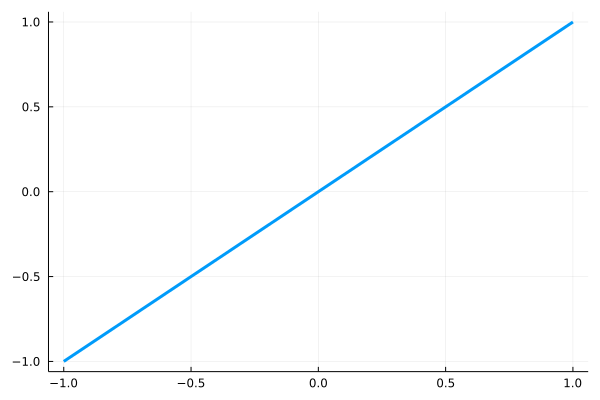
\includegraphics[width=\linewidth]{funciones-activacion/Identidad.png}
        \end{minipage}
        \\
        \hline
         %%%%%%%% Indicadora %%%%%%%
        % Nombre: 
        Indicadora $\lambda \in \R$
        & %expresión 
        $Indicadora_\lambda(x) = 1_{\{x > \lambda\}}$
        & % Rango imagen
        $\{0,1\}$
        & % Gráfica
        \begin{minipage}{\coeficienteAncho\textwidth}
            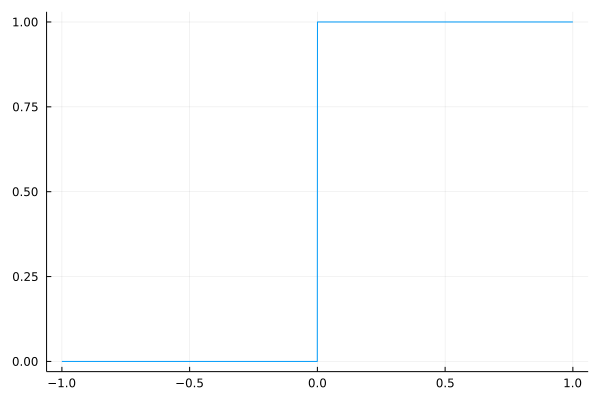
\includegraphics[width=\linewidth]{funciones-activacion/Indicadora de 0.png}
        \end{minipage}
        \\
        \hline
         %%%%%%%% Función umbral %%%%%%%
        % Nombre: 
        Función umbral $p$ polinomio
        & %expresión 
        $Threshold(x) = 1_{\{p(x) > 0\}}$
        & % Rango imagen
        $\{0,1\}$
        & % Gráfica
        \begin{minipage}{\coeficienteAncho\textwidth}
            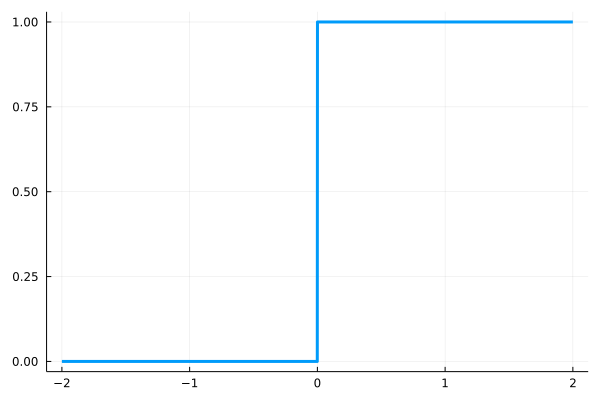
\includegraphics[width=\linewidth]{funciones-activacion/Threshold de polinomio 2x.png}
        \end{minipage}
        \\
        \hline
         %%%%%%%% Función rampa %%%%%%%
        % Nombre: 
        Función rampa
        & %expresión 
        $Rampa(x) = x 1_{\{0 < x <1\}} + 1_{\{x \geq 1\}}$ 
        & % Rango imagen
        $[0,1]$
        & % Gráfica
        \begin{minipage}{\coeficienteAncho\textwidth}
            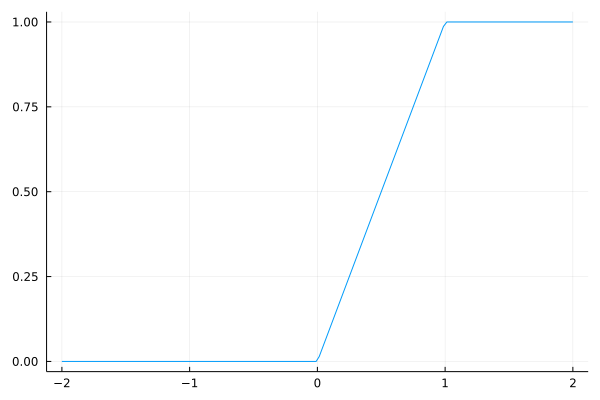
\includegraphics[width=\linewidth]{funciones-activacion/Rampa.png}
        \end{minipage}
        \\
        \hline
        %%%%%%%% sigmoide %%%%%%%%
        % Nombre: 
        Sigmoidea 
        & %expresión 
        $\sigma(x) = \frac{1}{1+e^{-x}}$
        & %Rango imagen
        $(0,1)$
        & % Gráfica
        \begin{minipage}{\coeficienteAncho\textwidth}
            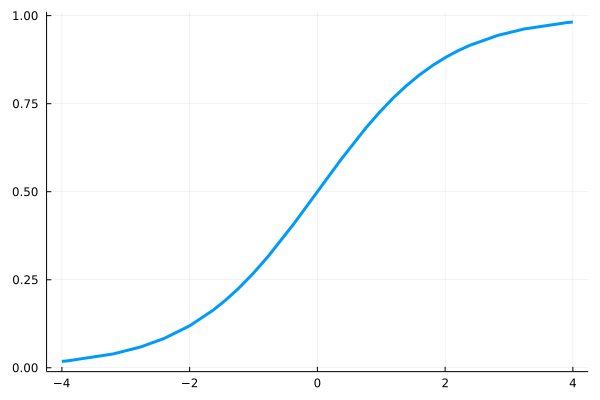
\includegraphics[width=\linewidth]{funciones-activacion/Sigmoid.png}
        \end{minipage}
        \\
        \hline
        %%%%%%%% Tangente hiperbólica  %%%%%%%%
        % Nombre: 
        Tangente hiperbólica 
        & %expresión 
        $\tanh$
        & %Rango imagen
        $(-1,1)$
        & % Gráfica
        \begin{minipage}{\coeficienteAncho\textwidth}
            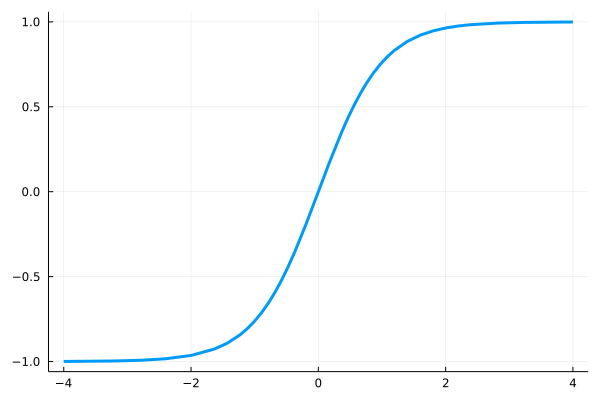
\includegraphics[width=\linewidth]{funciones-activacion/Tangente hiperbolica.png}
        \end{minipage}
        \\
        \hline
        %%%%%%%% Valor absoluto%%%%%%%%
        % Nombre: 
        Valor absoluto
        & %expresión 
        $abs(x)= |x|$
        & %Rango imagen
        $[0,+\infty]$
        & % Gráfica
        \begin{minipage}{\coeficienteAncho\textwidth}
            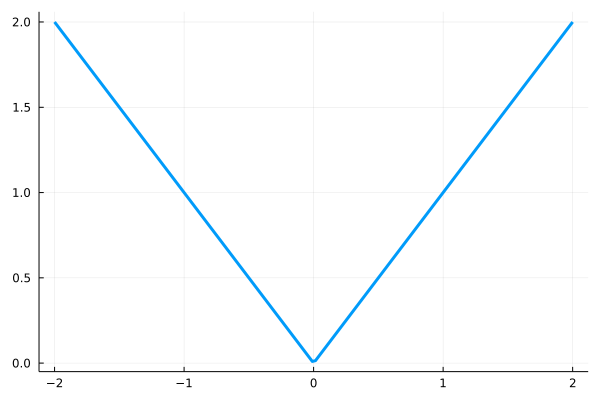
\includegraphics[width=\linewidth]{funciones-activacion/Valor absoluto.png}
        \end{minipage}
        \\
        \hline
         %%%%%%%% Coseno %%%%%%%%
        % Nombre: 
        Coseno
        & %expresión 
        $\cos$
        & %Rango imagen
        $[-1,1]$
        & % Gráfica
        \begin{minipage}{\coeficienteAncho\textwidth}
            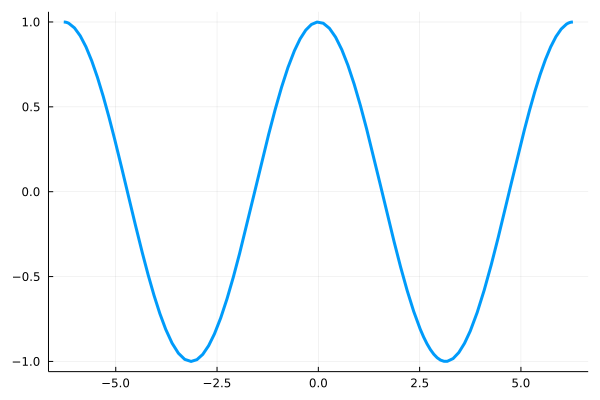
\includegraphics[width=\linewidth]{funciones-activacion/coseno.png}
        \end{minipage}
        \\
        \hline
        %%%%%%%% Cosine Squasher %%%%%%%%
        % Nombre: 
        \textit{Cosine Squasher}
        & %expresión 
        $CosineSquasher(x)=\left(1 + \cos\left(x + 3 \frac{\pi}{2} \right) \frac{1}{2}\right) 
        1_{\{\frac{-\pi}{2} \leq x \leq  \frac{\pi}{2}\}}
        +
        1_{\{ \frac{\pi}{2} < \lambda \}}.$
        & %Rango imagen
        $[0,1]$
        & % Gráfica
        \begin{minipage}{\coeficienteAncho\textwidth}
            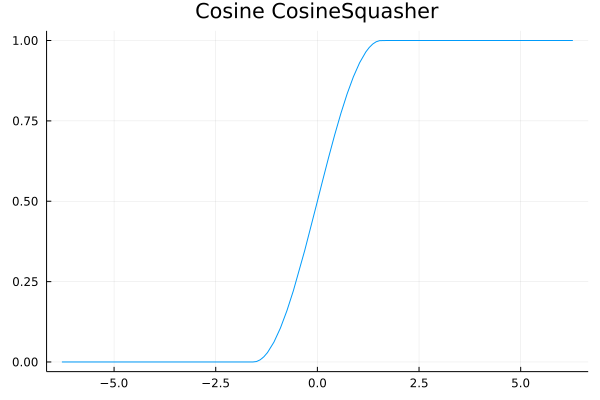
\includegraphics[width=\linewidth]{funciones-activacion/Cosine CosineSquasher.png}
        \end{minipage}
        \\
        \hline
        %%%%%%%% ReLU %%%%%%%%
        % Nombre: 
        \textit{ReLU}
        & %expresión 
        $ReLU(x) = \max(0,x)$
        & %Rango imagen
        $[0,+\infty)$
        & % Gráfica
        \begin{minipage}{\coeficienteAncho\textwidth}
            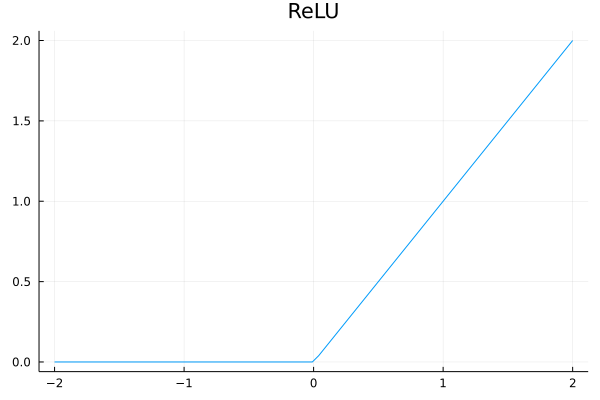
\includegraphics[width=\linewidth]{funciones-activacion/ReLU.png}
        \end{minipage}
        \\
        \hline
        %%%%%%%% Hard Hyperbolic Function %%%%%%%%
        % Nombre: 
        \textit{Hard Hyperbolic Function}
        & %expresión 
        $Hardtanh(x) =\left\{ \begin{array}{lcc}
            -1 &   si  & x \leq -1 \\
            \\ x &  si & -1< x < 1 \\
            \\ 1&  si  & x \geq 1 
            \end{array}
        \right.$
        & %Rango imagen
        $[-1,1]$
        & % Gráfica
        \begin{minipage}{\coeficienteAncho\textwidth}
            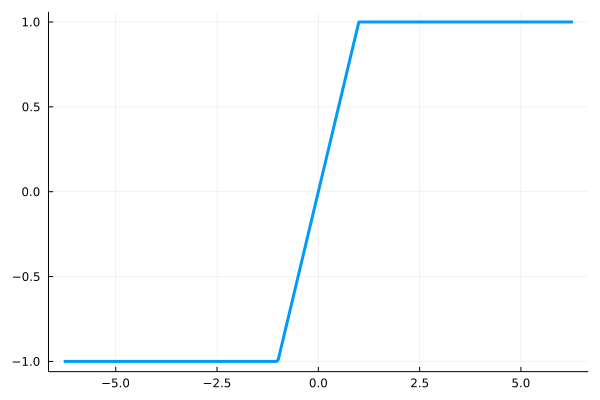
\includegraphics[width=\linewidth]{funciones-activacion/hardtanh.png}
        \end{minipage}
        \\
        \hline
        %%%%%%%% Leaky ReLU%%%%%%%
        % Nombre: 
        \textit{Leaky ReLU}
        & %expresión 
        $\begin{array}{c}

            LReLU_{\alpha}(x) =\left\{ \begin{array}{lcc}
            \alpha x &   si  & x \leq 0 \\
            \\ x&  si  & x > 0 
            \end{array}
            \right.
        \\
        \text{con } \alpha \in \R^+ \text{valor }\textit{pequeño}.
        \end{array}
        $
        & % Rango imagen
        $[0, +\infty)$
        & % Gráfica
        \begin{minipage}{\coeficienteAncho\textwidth}
            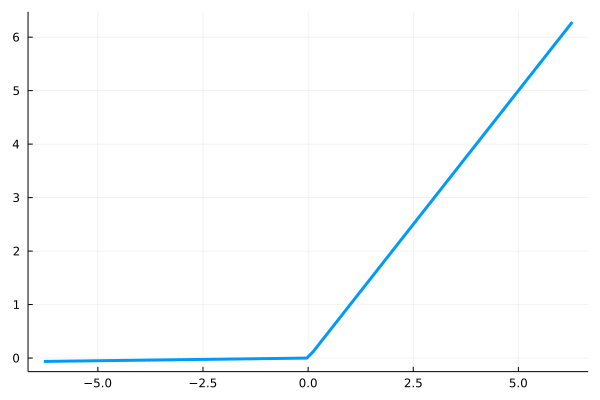
\includegraphics[width=\linewidth]{funciones-activacion/LReLU.png}
        \end{minipage}
        \\
        \hline
    \end{tabular}
    } % fin de llave de ajustarse al ancho de la página
    \caption{Compendio de funciones de activación}  
    \label{table:funciones-de-activation}
\end{table}

\begin{aportacionOriginal}

\begin{teorema}\label{teo:eficacia-funciones-activation}
    Sea $\phi \in \mathcal{A}(\R^2)$ una transformación afín, sean dos funciones de activación $\sigma, \gamma$ tales que 
    \begin{equation*}
        \phi \circ \sigma = \gamma,
    \end{equation*}
    entonces para 
    el espacio de redes neuronales de $n$ neuronas creado con la función de activación $\sigma$ es  
    igual al espacio de redes neuronales creado con la función de activación $\gamma$. 
\end{teorema}
\begin{proof}

    Sea $\mathcal{H}^+_{\sigma, n}(\R^d, \R^s)$, el espacio de redes neuronales con $n$ neuronas con sesgo. 

    Para cualquier $h  \in \mathcal{H}^+_{\sigma, n}(\R^d, \R^s)$
    la proyección i-ésima de $h$ será de la forma 

    \begin{equation*}
        h_i(x) = \sum^n_{j=1}(\beta_{j} \sigma(A_j(x))+ k_j),
    \end{equation*}
    con $x \in \R^d, \beta_{j}, k_j \in \R, A_j \in \afines$. 

    Procedemos a definir $\tilde{h}_i(x)$ como sigue y
    se tiene que 
    \begin{equation*}
        \tilde{h}_i(x) 
        = \sum^n_{j=1}(\beta_{j}  \phi(\sigma(A_j(x)))+ k_j)
        = \sum^n_{j=1}(\tilde{\beta}_{j} \sigma(\tilde{A}_j(x))+ \tilde{k_j}),
    \end{equation*}
    con $x \in \R^d, \tilde \beta_{j}, \tilde k_j \in \R, \tilde{A}_j \in \afines$,
    por lo que está claro que $\tilde{h}_i(x) \in \mathcal{H}^+_{\sigma, n}(\R^d, \R^s)$. 

    Pero por hipótesis del teorema $\phi \circ \sigma = \gamma$, por lo que $\tilde{h}_i(x) \in \mathcal{H}^+_{\gamma, n}(\R^d, \R^s)$. 

    Basta con considerar la transformación afín inversa para ver que ambos espacios son isomorfos
    \begin{equation*}
        \mathcal{H}^+_{\gamma, n}(\R^d, \R^s) \simeq \mathcal{H}^+_{\sigma, n}(\R^d, \R^s).
    \end{equation*}

    Dos conjuntos isomorfos donde para cualquier $h \in \mathcal{H}^+_{\gamma, n}(\R^d, \R^s)$, 
    se tiene que $h \in \mathcal{H}^+_{\sigma, n}(\R^d, \R^s)$ via el isomorfismo y 
    luego componer con la inversa de la aplicación afín. 

    Como demostramos en \ref{consideration-irrelevancia-sesgo} se tiene que 
    \begin{equation*}
        \mathcal{H}^+_{\sigma, n}(\R^d, \R^s) = \mathcal{H}^+_{\gamma, n}(\R^d, \R^s) 
        \subset 
            \mathcal{H}_{\gamma, n+1}(\R^d, \R^s) 
        \subset
        \mathcal{H}^+_{\gamma, {n+1}}(\R^d, \R^s) = \mathcal{H}^+_{\sigma, {n+1}}(\R^d, \R^s) 
        .
    \end{equation*}
    Por lo que para un $n$ arbitrariamente grande, se acaba de probar lo buscado. 
    \begin{equation*}
        \mathcal{H}_{\gamma}(\R^d, \R^s) = \mathcal{H}_{\sigma}(\R^d, \R^s).
    \end{equation*}
\end{proof}
\end{aportacionOriginal}

\subsubsection*{Relevancia práctica del teorema}
Este teorema lo que nos está diciendo es que si dos funciones de activación tienen \textit{la misma forma}
(independientemente de su grafo)
entonces \textbf{aproximarán igual de bien},
es decir, con el mismo error dentro de un conjunto de datos.
 Esto a nivel práctico  significa que \textbf{si se tienen dos funciones de activación
  \textit{con la misma forma} (o muy parecidas) elige
   la que tenga menor costo computacional}, porque a 
   nivel teórico aproximarán igual de bien y de esta
    manera ahorraremos recursos. 

Notemos además que la demostración nos enseña que la igualdad se da independientemente del número de 
neuronas fijado, es decir que no es un resultado 
asintótico (lo asintótico en términos prácticos 
significa que sea resultado de una serie de 
aproximaciones).  


Así pues a la vista de la imágenes de las distintas funciones de activación 
recogidas en la tabla \ref{table:funciones-de-activation} y
por el recién probado teorema \ref{teo:eficacia-funciones-activation} podemos determinar a priori 
que de manera teórica existen conjuntos de funciones que aproximadamente  puedes producir los mismos resultado, 
compararemos entonces su coste computacional y tomaremos como representante de la clase aquel que sea de menor coste. 

\begin{table}[H] 
    \centering  
    \begin{tabular}{| c | c | c | }
        \hline
        \textit{Grupo escalera} & \textit{Grupo sigmoide} & \textit{Grupo ReLU} \\
        \hline
       &  Rampa &  \\
       Indicadora & Sigmodea & ReLU\\
       Umbral & \textit{Cosine Squasher}& LReLU\\
        & tanh & \\
        & \textit{Hard Hyperbolic Function}& \\
\hline
    \end{tabular}
    \caption{Agrupaciones de funciones de activación con forma similar}  
    \label{table:Clases-equivalencia-activation-function}
\end{table}

\subsection{ Implementación de las funciones de activación en la biblioteca de redes neuronales} 

Las funciones de activación han sido implementadas con cuidado de que sean eficientes 
y valiéndose de las características propias de Julia, para ello se han utilizado técnicas como: 

\begin{itemize}
    \item \textbf{Programación modular}: Tal y como se recomienda en la documentación de Julia \footnote{
        Consultada en la página web oficial de Julia  a día 23 de mayo del 2022 con URL: \url{https://docs.julialang.org/en/v1/manual/modules/}
    } se ha utilizado una módulo en la implementación de la biblioteca, esto aporta los siguientes beneficios: 
    \begin{itemize}
        \item Los módulos pueden ser precompilados y de esta manera se aceleraría la carga y el tiempo de inicialización. 
        \item Encapsulamiento de los métodos y facilidades de uso del espacio de nombres, lo cual forma parte
        de una buena metodología de programación. 
    \end{itemize}
    \item \textbf{Macros}\footnote{La información consultada de macros ha sido  de la página oficial de Julia, a día 23 de mayo del 2022, URL:
    \url{https://docs.julialang.org/en/v1/manual/metaprogramming}}:
    que permiten sustituciones de código cuando el código es analizado por el compilador, 
    de esta manera, funciones que devuelven otras funciones dependientes de un parámetro se verán beneficiadas. 
     Puede encontrar la implementación de esto en la biblioteca de redes neuronales implementada en nuestro 
     repositorio \footnote{Esto es en \url{https://github.com/BlancaCC/TFG-Estudio-de-las-redes-neuronales/tree/main/Biblioteca-Redes-Neuronales/src/activation_functions.jl}}
\end{itemize}




\subsection{Coste computacional funciones activación }

\subsubsection{Diseño del experimento}
El experimento para comparar los resultados ha consistido: 
Se ha evaluado cada función a comparar $20000000$ veces y se ha medido cuanto tarda. 
Esto se ha repetido $15$ veces. Puede encontrar la implementación concreta y los resultados concretos de cada iteración en el repositorio del
proyecto \footnote{En el directorio de experimentos 
de \url{https://github.com/BlancaCC/TFG-Estudio-de-las-redes-neuronales}.}.

\subsubsection{Test de hipótesis}

Compararemos si los resultados son significativos utilizando la \textbf{prueba de los rangos con 
signo de Wilcoxon} (véase \cite{OpenIntroStatistics}, \cite{BiologicalStatistics}, o la web de \href{https://www.cienciadedatos.net}{cienciadedatos.net} \footnote{
 Prueba de los rangos con signo de Wilcoxon by Joaquín Amat Rodrigo, available under a Attribution 4.0 International (CC BY 4.0) at
  \url{https://www.cienciadedatos.net/documentos/18_prueba_de_los_rangos_con_signo_de_wilcoxon}
  Con fecha de visita el 22 de mayo del 2022.
  }).

  La motivación de realizar esta prueba es la siguiente: 
\begin{itemize}
    \item Las muestras son independientes.
    \item Los datos tomados, el tiempo, permiten ser ordenados. 
    \item El tamaño de muestra es pequeño y no podemos asegurar normalidad de la datos. 
\end{itemize}

\subsubsection*{Hipótesis} 

\begin{itemize}
    \item $H_0$: La mediana de las diferencia de cada par de datos es $0$. 
    \item $H_a$: La mediana de las diferencia entre cada par de datos es diferente de cero. 
\end{itemize}

La utilidad de este test es que si rechaza la hipótesis la hipótesis nula sabremos que con un $95 \%$ de certeza tendrán medianas diferentes, es decir, \textbf{existe una 
diferencia de tiempos}. En caso de que no se rechace no podremos afirmar nada.
Puede encontrar la implementación en el repositorio del
 proyecto \footnote{En el directorio de experimentos 
 de \url{https://github.com/BlancaCC/TFG-Estudio-de-las-redes-neuronales}.}.

 Los resultados del test de Wilcoxon han sido los siguientes: 

 \begin{table}[H]
    \resizebox{\textwidth}{!}{
    \begin{tabular}{|l|l|l|l|l|l|}
    \hline
        ~ & cte 1  & Identidad  & Threshold de $2x$ & CosineSquasher & Indicadora de 0 \\ \hline
        cte 1  & - &\textbf{No rechaza $H_0$} & Rechaza $H_0$ & Rechaza $H_0$ & Rechaza $H_0$ \\ \hline
        Identidad  & \textbf{No rechaza $H_0$} & - & Rechaza $H_0$ & Rechaza $H_0$ & Rechaza $H_0$ \\ \hline
        Threshold de $2x$ & Rechaza $H_0$ & Rechaza $H_0$ & - & Rechaza $H_0$ & \textbf{No rechaza $H_0$} \\ \hline
        CosineSquasher & Rechaza $H_0$ & Rechaza $H_0$ & Rechaza $H_0$ & - & Rechaza $H_0$ \\ \hline
        Indicadora de 0 & Rechaza $H_0$ & Rechaza $H_0$ & \textbf{No rechaza $H_0$} & Rechaza $H_0$ & - \\ \hline
        Rampa & Rechaza $H_0$ & Rechaza $H_0$ & \textbf{No rechaza $H_0$} & Rechaza $H_0$ & Rechaza $H_0$ \\ \hline
        ReLU & Rechaza $H_0$ & Rechaza $H_0$ & \textbf{No rechaza $H_0$} & Rechaza $H_0$ & \textbf{No rechaza $H_0$} \\ \hline
        Sigmoid & Rechaza $H_0$ & Rechaza $H_0$ & Rechaza $H_0$ & Rechaza $H_0$ & Rechaza $H_0$ \\ \hline
        Tangente hiperbólica & Rechaza $H_0$ & Rechaza $H_0$ & Rechaza $H_0$ & Rechaza $H_0$ & Rechaza $H_0$ \\ \hline
        Valor absoluto & Rechaza $H_0$ & Rechaza $H_0$ & Rechaza $H_0$ & Rechaza $H_0$ & Rechaza $H_0$ \\ \hline
        Coseno & Rechaza $H_0$ & Rechaza $H_0$ & Rechaza $H_0$ & Rechaza $H_0$ & Rechaza $H_0$ \\ \hline
        Hardtanh & Rechaza $H_0$ & Rechaza $H_0$ & Rechaza $H_0$ & Rechaza $H_0$ & Rechaza $H_0$ \\ \hline
        LReLU & Rechaza $H_0$ & Rechaza $H_0$ & \textbf{No rechaza $H_0$} & Rechaza $H_0$ & \textbf{No rechaza $H_0$} \\ \hline
    \end{tabular}
    }
    \caption{Resultados 1 de 3: Rechazos con un $95\%$ de confianza en el test Wilcoxon.}
    \label{Rechazo-1-de-3}
\end{table}

\begin{table}[H]
    \resizebox{\textwidth}{!}{
    \begin{tabular}{|l|l|l|l|l|}
    \hline
        ~ & Rampa & ReLU & Sigmoid & Tangente hiperbólica \\ \hline
        cte 1  & Rechaza $H_0$ & Rechaza $H_0$ & Rechaza $H_0$ & Rechaza $H_0$ \\ \hline
        Identidad  & Rechaza $H_0$ & Rechaza $H_0$ & Rechaza $H_0$ & Rechaza $H_0$ \\ \hline
        Threshold de $2x$ & \textbf{No rechaza $H_0$} & \textbf{No rechaza $H_0$} & Rechaza $H_0$ & Rechaza $H_0$ \\ \hline
        CosineSquasher & Rechaza $H_0$ & Rechaza $H_0$ & Rechaza $H_0$ & Rechaza $H_0$ \\ \hline
        Indicadora de 0 & Rechaza $H_0$ & \textbf{No rechaza $H_0$} & Rechaza $H_0$ & Rechaza $H_0$ \\ \hline
        Rampa & - & \textbf{No rechaza $H_0$} & Rechaza $H_0$ & Rechaza $H_0$ \\ \hline
        ReLU & \textbf{No rechaza $H_0$} & - & Rechaza $H_0$ & Rechaza $H_0$ \\ \hline
        Sigmoid & Rechaza $H_0$ & Rechaza $H_0$ & - & Rechaza $H_0$ \\ \hline
        Tangente hiperbólica & Rechaza $H_0$ & Rechaza $H_0$ & Rechaza $H_0$ & - \\ \hline
        Valor absoluto & Rechaza $H_0$ & Rechaza $H_0$ & Rechaza $H_0$ & Rechaza $H_0$ \\ \hline
        Coseno & Rechaza $H_0$ & Rechaza $H_0$ & Rechaza $H_0$ & Rechaza $H_0$ \\ \hline
        Hardtanh & Rechaza $H_0$ & Rechaza $H_0$ & Rechaza $H_0$ & Rechaza $H_0$ \\ \hline
        LReLU & \textbf{No rechaza $H_0$} & \textbf{No rechaza $H_0$} & Rechaza $H_0$ & Rechaza $H_0$ \\ \hline
    \end{tabular}
    }
    \caption{Resultados 2 de 3: Rechazos con un $95\%$ de confianza en el test Wilcoxon.}
    \label{Rechazo-2-de-3}
\end{table}

\begin{table}[H]
    \resizebox{\textwidth}{!}{
    \begin{tabular}{|l|l|l|l|l|}
    \hline
        ~ & Valor absoluto & Coseno & Hardtanh & LReLU \\ \hline
        cte 1  & Rechaza $H_0$ & Rechaza $H_0$ & Rechaza $H_0$ & Rechaza $H_0$ \\ \hline
        Identidad  & Rechaza $H_0$ & Rechaza $H_0$ & Rechaza $H_0$& Rechaza $H_0$ \\ \hline
        Threshold de $2x$ & Rechaza $H_0$ & Rechaza $H_0$ & Rechaza $H_0$ & \textbf{No rechaza $H_0$} \\ \hline
        CosineSquasher & Rechaza $H_0$ & Rechaza $H_0$ & Rechaza $H_0$ & Rechaza $H_0$ \\ \hline
        Indicadora de 0 & Rechaza $H_0$ & Rechaza $H_0$ & Rechaza $H_0$ & \textbf{No rechaza $H_0$} \\ \hline
        Rampa & Rechaza $H_0$& Rechaza $H_0$ & Rechaza $H_0$ & \textbf{No rechaza $H_0$} \\ \hline
        ReLU & Rechaza $H_0$ & Rechaza $H_0$ & Rechaza $H_0$ & \textbf{No rechaza $H_0$} \\ \hline
        Sigmoid & Rechaza $H_0$ & Rechaza $H_0$ & Rechaza $H_0$ & Rechaza $H_0$ \\ \hline
        Tangente hiperbólica & Rechaza $H_0$ & Rechaza $H_0$ & Rechaza $H_0$ & Rechaza $H_0$ \\ \hline
        Valor absoluto & - & Rechaza $H_0$ & Rechaza $H_0$ & \textbf{No rechaza $H_0$} \\ \hline
        Coseno & Rechaza $H_0$ & - & Rechaza $H_0$ & Rechaza $H_0$ \\ \hline
        Hardtanh & Rechaza $H_0$ & Rechaza $H_0$ & - & Rechaza $H_0$ \\ \hline
        LReLU & Rechaza $H_0$ & \textbf{No rechaza $H_0$} & Rechaza $H_0$ & - \\ \hline
    \end{tabular}
    }
    \caption{Resultados 3 de 3: Rechazos con un $95\%$ de confianza en el test Wilcoxon.}
    \label{Rechazo-3-de-3}
\end{table}

Como ya comentábamos, si la hipótesis nula es rechazada podemos suponer que hay una diferencia 
de tiempo significativas;  en caso contrario no podemos saber nada. 

Sin embargo podemos entender estos rechazos como una clase de equivalencia; es decir, la diferencia en coste computacional no es tan significativa, dentro de ese grupo. De hecho, como podemos apreciar en la tabla \ref{Tiempos-ejecucion-comparativas}, que está ordenada de menor tiempo a mayor,
 estos se encuentra en posiciones consecutivas.

\begin{table}[H]
    \centering
    \begin{tabular}{|l|l|l|l|}
    \hline
        Función & Mediana & Media Tiempo & Desviación típica \\ \hline
        cte 1 (para comparar) & 1475,959 & 1473,478 & 26,332 \\ \hline
        Identidad (para comparar) & 1479,817 & 1467,311 & 27,021 \\ \hline
        Hardtanh & 1495,105 & 1491,046 & 21,334 \\ \hline
        CosineSquasher & 1522,128 & 1521,117 & 19,223 \\ \hline
        ReLU & 1546,379 & 1552,049 & 21,435 \\ \hline
        Indicadora de 0 & 1554,432 & 1556,114 & 21,814 \\ \hline
        Rampa & 1557,449 & 1552,169 & 25,043 \\ \hline
        Threshold de $2x$ & 1562,809 & 1556,669 & 23,029 \\ \hline
        LReLU & 1564,124 & 1561,367 & 21,722 \\ \hline
        Valor absoluto & 1583,266 & 1580,545 & 23,464 \\ \hline
        Sigmoid & 1608,797 & 1601,079 & 21,938 \\ \hline
        Coseno & 1630,392 & 1629,634 & 26,113 \\ \hline
        Tangente hiperbólica & 1664,006 & 1653,295 & 23,025 \\ \hline
    \end{tabular}
    \caption{Tiempo de ejecución en segundos}
    \label{Tiempos-ejecucion-comparativas}
\end{table}


Si volvemos a nuestro objetivo, que era encontrar el representante de 
menor costo entre las agrupaciones dispuestas en la tabla \ref{table:Clases-equivalencia-activation-function}. Concluimos que los mejores candidatos son: 

\begin{itemize}
    \item Para el \textit{grupo escalera}: No se ha rechazado la hipótesis nula, luego a priori no hay deferencia significativa y podemos seleccionar el candidato que queramos. 
    \item Para el \textit{grupo sigmoide}: La mejor opción ha sido \textit{Hard Hyperbolic Function} y  después en orden de mejor a peor: \textit{Cosine Squasher}, rampa, sigmodea y tangente hiperbólica.
    \item Pare el \textit{grupo ReLU}: No se ha rechazado la hipótesis nula, así que no podemos decir nada. 
\end{itemize}

